% Template for PLoS
% Version 3.1 February 2015
%
% To compile to pdf, run:
% latex plos.template
% bibtex plos.template
% latex plos.template
% latex plos.template
% dvipdf plos.template
%
% % % % % % % % % % % % % % % % % % % % % %
%
% -- IMPORTANT NOTE
%
% This template contains comments intended 
% to minimize problems and delays during our production 
% process. Please follow the template instructions
% whenever possible.
%
% % % % % % % % % % % % % % % % % % % % % % % 
%
% Once your paper is accepted for publication, 
% PLEASE REMOVE ALL TRACKED CHANGES in this file and leave only
% the final text of your manuscript.
%
% There are no restrictions on package use within the LaTeX files except that 
% no packages listed in the template may be deleted.
%
% Please do not include colors or graphics in the text.
%
% Please do not create a heading level below \subsection. For 3rd level headings, use \paragraph{}.
%
% % % % % % % % % % % % % % % % % % % % % % %
%
% -- FIGURES AND TABLES
%
% Please include tables/figure captions directly after the paragraph where they are first cited in the text.
%
% DO NOT INCLUDE GRAPHICS IN YOUR MANUSCRIPT
% - Figures should be uploaded separately from your manuscript file. 
% - Figures generated using LaTeX should be extracted and removed from the PDF before submission. 
% - Figures containing multiple panels/subfigures must be combined into one image file before submission.
% For figure citations, please use "Fig." instead of "Figure".
% See http://www.plosone.org/static/figureGuidelines for PLOS figure guidelines.
%
% Tables should be cell-based and may not contain:
% - tabs/spacing/line breaks within cells to alter layout or alignment
% - vertically-merged cells (no tabular environments within tabular environments, do not use \multirow)
% - colors, shading, or graphic objects
% See http://www.plosone.org/static/figureGuidelines#tables for table guidelines.
%
% For tables that exceed the width of the text column, use the adjustwidth environment as illustrated in the example table in text below.
%
% % % % % % % % % % % % % % % % % % % % % % % %
%
% -- EQUATIONS, MATH SYMBOLS, SUBSCRIPTS, AND SUPERSCRIPTS
%
% IMPORTANT
% Below are a few tips to help format your equations and other special characters according to our specifications. For more tips to help reduce the possibility of formatting errors during conversion, please see our LaTeX guidelines at http://www.plosone.org/static/latexGuidelines
%
% Please be sure to include all portions of an equation in the math environment.
%
% Do not include text that is not math in the math environment. For example, CO2 will be CO\textsubscript{2}.
%
% Please add line breaks to long display equations when possible in order to fit size of the column. 
%
% For inline equations, please do not include punctuation (commas, etc) within the math environment unless this is part of the equation.
%
% % % % % % % % % % % % % % % % % % % % % % % % 
%
% Please contact latex@plos.org with any questions.
%
% % % % % % % % % % % % % % % % % % % % % % % %

\documentclass[10pt,letterpaper]{article}
\usepackage[top=0.85in,left=2.75in,footskip=0.75in]{geometry}

% Use adjustwidth environment to exceed column width (see example table in text)
\usepackage{changepage}

% Use Unicode characters when possible
\usepackage[utf8]{inputenc}

% textcomp package and marvosym package for additional characters
\usepackage{textcomp,marvosym}

% fixltx2e package for \textsubscript
\usepackage{fixltx2e}

% amsmath and amssymb packages, useful for mathematical formulas and symbols
\usepackage{amsmath,amssymb}

% cite package, to clean up citations in the main text. Do not remove.
\usepackage{cite}

% Use nameref to cite supporting information files (see Supporting Information section for more info)
\usepackage{nameref,hyperref}

% line numbers
\usepackage[right]{lineno}

% ligatures disabled
\usepackage{microtype}
\DisableLigatures[f]{encoding = *, family = * }

% rotating package for sideways tables
\usepackage{rotating}

\usepackage{verbatim}   % useful for program listings

% Remove comment for double spacing
%\usepackage{setspace} 
%\doublespacing

% Text layout
\raggedright
\setlength{\parindent}{0.5cm}
\textwidth 5.25in 
\textheight 8.75in

% Bold the 'Figure #' in the caption and separate it from the title/caption with a period
% Captions will be left justified
\usepackage[aboveskip=1pt,labelfont=bf,labelsep=period,justification=raggedright,singlelinecheck=off]{caption}

% Use the PLoS provided BiBTeX style
% \bibliographystyle{plos2015}
\bibliographystyle{apalike}

% Remove brackets from numbering in List of References
\makeatletter
\renewcommand{\@biblabel}[1]{\quad#1.}
\makeatother

% Leave date blank
\date{}

% Header and Footer with logo
\usepackage{lastpage,fancyhdr,graphicx}
\usepackage{epstopdf}
\pagestyle{myheadings}
\pagestyle{fancy}
\fancyhf{}
\lhead{
\includegraphics[width=2.0in]{PLOS-submission.eps}}
\rfoot{\thepage/\pageref{LastPage}}
\renewcommand{\footrule}{\hrule height 2pt \vspace{2mm}}
\fancyheadoffset[L]{2.25in}
\fancyfootoffset[L]{2.25in}
\lfoot{\sf PLOS}

%% Include all macros below

\newcommand{\lorem}{{\bf LOREM}}
\newcommand{\ipsum}{{\bf IPSUM}}

%% END MACROS SECTION


\begin{document}
\vspace*{0.35in}

% Title must be 250 characters or less.
% Please capitalize all terms in the title except conjunctions, prepositions, and articles.
\begin{flushleft}
{\Large
\textbf\newline{Filament Recycling and Sustained Contractile Flows in an Actomyosin Cortex}
}
\newline
% Insert author names, affiliations and corresponding author email (do not include titles, positions, or degrees).
\\
William McFadden\textsuperscript{1},
Jonathan Michaux\textsuperscript{2},
Patrick McCall\textsuperscript{3},
Edwin Munro\textsuperscript{2,*}
\\
\bigskip
\bf{1} Biophysical Sciences Program, University of Chicago, Chicago, IL, USA
\\
\bf{2} Department of Molecular Genetics and Cell Biology, University of Chicago, Chicago, IL, USA
\\
\bf{3} Department of Physics, University of Chicago, Chicago, IL, USA
\\
\bigskip

% Insert additional author notes using the symbols described below. Insert symbol callouts after author names as necessary.
% 
% Remove or comment out the author notes below if they aren't used.
%
% Primary Equal Contribution Note
%\Yinyang These authors contributed equally to this work.

% Additional Equal Contribution Note
% Also use this double-dagger symbol for special authorship notes, such as senior authorship.
%\ddag These authors also contributed equally to this work.

% Current address notes
%\textcurrency a Insert current address of first author with an address update
% \textcurrency b Insert current address of second author with an address update
% \textcurrency c Insert current address of third author with an address update

% Deceased author note
%\dag Deceased

% Group/Consortium Author Note
%\textpilcrow Membership list can be found in the Acknowledgments section.

% Use the asterisk to denote corresponding authorship and provide email address in note below.
* emunro@uchicago.edu

\end{flushleft}
% Please keep the abstract below 300 words
\section*{Abstract}
Fill in abstract later.


% Please keep the Author Summary between 150 and 200 words
% Use first person. PLOS ONE authors please skip this step. 
% Author Summary not valid for PLOS ONE submissions.   
\section*{Author Summary}
In this paper, we develop and analyze a minimal model for 2D active networks based on the cortical cytoskeleton of eukaryotic embryos.  Our model introduces a drag-like slip between cross-linked filaments as means to dissipate stored stress, generating a macroscopic effective viscosity.  We further introduce an active friction to active stress from microscopic properties.  We generate computational simulations based on the model, and demonstrate that active stress is sufficient to drive network contraction only temporarily.  By introducing filament recycling, we are able to set up steady state flow profiles such as those found in the cortex of developing embryos and migrating cells.  The model is used to calculate phenomenological constants measured in prior experiments.  Our analysis sheds insight on potential microscopic control parameters governing broad qualitative differences in 2D active networks.  We make our model freely accessible and our methodology transparent to enable other researchers to clearly understand our modeling framework and to build upon our findings.

\linenumbers

\section*{Introduction}

\paragraph{}  Cortical flow is a fundamental and ubiquitous form of cellular deformation that underlies cell polarization, cell division, cell crawling and multicellular tissue morphogenesis\cite{cellmech_flows3,cellmech_flows2}.  These flows arise within the actomyosin cortex, a thin layer of cross-linked actin filaments and myosin motors that lies just beneath the plasma membrane \cite{Salbreux2012536}. The active forces that drive cortical flows are thought to be generated by myosin motors pulling against individual actin filaments \cite{Munro2004413}. These forces must be integrated within cross-linked networks to build macroscopic contractile stress.  At the same time, cross-linked networks resist deformation and this resistance must be dissipated by network remodeling to allow macroscopic network deformation and flow.  How force production and dissipation depend on motor activity, network architecture and remodeling remains poorly understood.

Current models for cortical flow rely on coarse-grained descriptions of actomyosin networks as active fluids, whose motions are driven by gradients of active contractile stress and opposed by an effectively viscous resistance\cite{cellmech_flows}.  In these models, gradients of active stress are assumed to reflect spatial variation in motor activity and viscous resistance is assumed to reflect the internal dissipation of elastic resistance due to local remodeling of filaments and/or crosslinks \cite{PhysRevLett.106.028103}.  A key virtue of these models is that their behavior is governed by a few parameters (active stress and effective viscosity).  By coupling an active fluid description to simple kinetic models for network assembly and disassembly and making active stress and effective viscosity depend on e.g network density and turnover rates, it is possible to capture phenomenological descriptions of cortical flow.  Models based on this active fluids description can successfully reproduce spatiotemporal dynamics of cortical flow observed during polarization \cite{cellmech_flows}, cell division \cite{Turlier2014114,PhysRevLett.103.058102}, cell motility \cite{Keren:2009aa,RevModPhys.85.1143} and tissue morphogenesis \cite{Heisenberg2013948}.  

However, to understand how cells exert physiological control over cortical deformation and flow, or to build and tune networks with desired properties {\em in vitro}, it is essential to connect this coarse-grained description to the microscopic origins of force generation and dissipation within cross-linked actomyosin networks.  Both active stress and effective viscosity depend sensitively on microscopic parameters including densities of filaments, motors and cross-links, force-dependent motor/filament interactions, cross-link dynamics and network turnover rates.  Thus a key challenge is to understand how tuning these microscopic parameters controls the dynamic interplay between active force generation and passive relaxation to control macroscopic dynamics of cortical flow.

\paragraph{} Studies in living cells have documented fluid-like stress relaxation on timescales of 10-100s of seconds \cite{cellmech_flows,cellmech_flows2,cellmech_flows3,rheo_fluid,rheo_fluid2,cell_rheo_exp}.  These modes of stress relaxation are thought to arise both from the transient binding/unbinding of individual cross-links and from the turnover (assembly/disassembly) of actin filaments (ref).  Studies of cross-linked and/or bundled actin networks {\em in vitro} suggest that cross-link unbinding may be sufficient to support viscous relaxation (creep) on very long timescales\cite{rheo_crosslinksmatter,rheo_crosslinkslip1,rheo_crosslinkslip2,rheo_crosslinkslip3,rheo_nonaffine}, but is unlikely to explain the rapid large scale cortical deformation and flow observed in living cells.  suggest that rapid actin turnover must play a significant role as well. Indeed, photokinetic and single molecule imaging studies studies reveal rapid turnover of cortical actin filaments in living cells on timescales of 10-100 seconds \cite{Robin:2014aa}. Previous theoretical models have explored  the dependence of stress relaxation on cross-link binding and unbinding analytically \cite{theo_crosslinkslip1,theo_crosslinkslip2} and others have explicitly modeled reversible cross-linking in combination with complex mechanics of filament bundles \cite{model_taeyoon,rheo_crosslinkslip2,theo_crosslinkslip3}.  However, until very recently \cite{Mak:2016aa} very little attention has been paid to actin turnover as mechanism of stress relaxation. 

Recent work has also begun to reveal insights into mechanisms that govern active stress generation in disordered actomyosin networks. In vitro studies have confirmed that local interactions among actin filaments and myosin motors are sufficient to drive macroscopic contraction of disordered networks \cite{rheo_2D1}.  Theoretical studies suggest that asymmetrical compliance of actin filaments (stiffer under extension than compression) and spatial differences (dispersion) in motor activity are sufficient conditions for contraction in one \cite{1367-2630-14-3-033037} and two \cite{PhysRevX.4.041002} dimensional networks, although other routes to contractility may also exist \cite{PhysRevX.4.041002}.  Further work has explored how modulation of network architecture, crosslink dynamics and motor density, activity and assembly state can shape rates and patterns of network deformation \cite{10.1371/journal.pone.0039869,Alvarado:2013aa,C0SM00494D} or network rheology \cite{0295-5075-85-1-18007,rheo_active}.  

Significantly, {\em in vitro} models for disordered actomyosin networks have used stable actin filaments, and these networks  support only transient contraction, either because of network collapse (ref), or buildup of elastic resistance (ref?), or because network rearrangements (polarity sorting) dissipate the potential to generate contractile force (ref). This suggest that continuous turnover of actin filaments may play a key role in allowing sustained deformation and flow (refs). Recent theoretical and modeling studies have begun to explore how this could work \cite{2015arXiv150706182H,Mak:2016aa,10.1371/journal.pone.0000696}, and to explore dynamic behaviors that can emerge in contractile material with turnover \cite{PhysRevLett.113.148102}. However, there is much to learn about how the buildup and maintenance of contractile force during continuous deformation and flow depends local interplay of network architecture, motor activity and filament turnover.

\paragraph{}  The goal of this work was to build a computational bridge between the microscopic description of cross-linked actomyosin networks and the coarse grained macroscopic description of an active fluid.  We sought to capture the essential microscope features (dynamic cross-links, active motors and semi flexible actin filaments with asymmetric compliance and continuous filament recycling), but in a way that is sufficiently simple to allow systematic exploration of how parameters that govern network deformation and flow in an active fluid theory depend on microscopic parameters. To this end, we introduce several coarse-grained approximations into our representation of filament networks. First, we represent semi-flexible actin filaments as chains of simple springs with asymmetric compliance (stronger in extension than compression). Second, we replace  dynamic binding/unbinding of elastic cross-links with a coarse-grained representation in terms of molecular friction \cite{theo_friction,theo_frictionSam,theo_molefric}, such that filaments can slide past each other against a constant fictional resistance. Third, we used a similar scheme to introduce active motors at filament crossover points with a simple linear force/velocity relationship, and we introduce ?dispersion? of motor activity by making only a subset of filament overlaps active \cite{theo_frictionShila}.  Finally, we model filament turnover by regularly reseting a subset of filaments to a new unstrained position. Importantly, these simplification allows us to extend our single polymer models to dynamical systems of larger network models for direct comparison between theory and modeling results. This level of coarse graining will therefore make it easier to understand classes of behavior for varying compositions of cross-linked filament networks. In addition, it allows us to compute a new class of numerical simulations efficiently, which gives us concrete predictions for behaviors in widely different networks with measurable dependencies on molecular details. 
  

% You may title this section "Methods" or "Models". 
% "Models" is not a valid title for PLoS ONE authors. However, PLoS ONE
% authors may use "Analysis" 
\section*{Models}

\begin{figure}[h!]
\centering
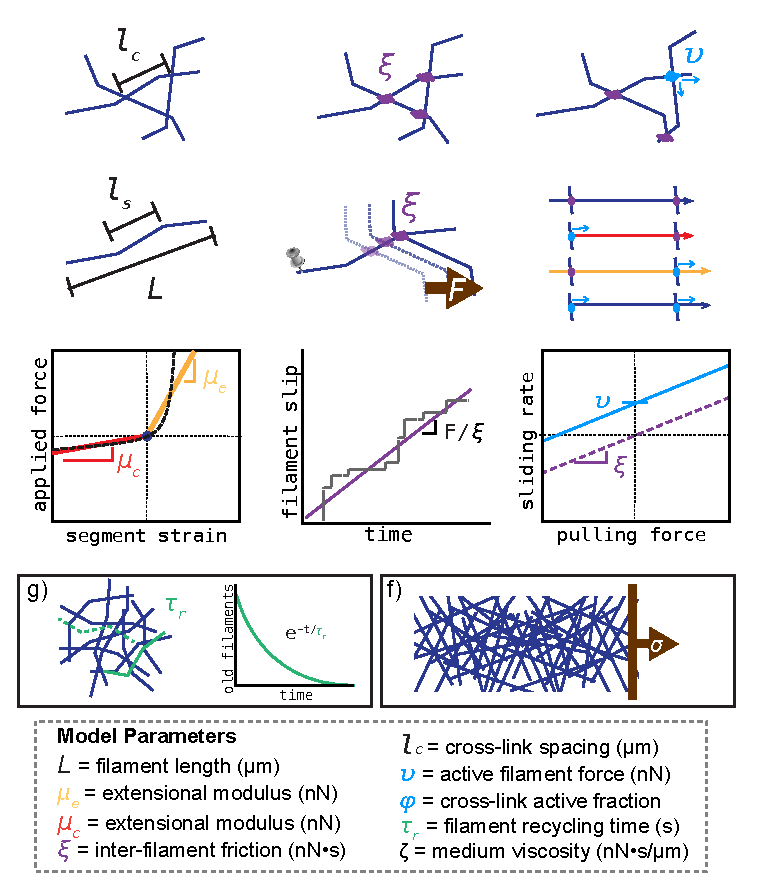
\includegraphics[width=\hsize]{figures/fig2/fig2}
\caption{\label{fig:sim} Schematic of modeling framework. a) Filaments are represented as connected chains of spring-like segments with asymmetric compliance.segments have a smaller spring constant for compression than for extension. b) Cross-linking is represented as filament coupling by an effective drag, such that their relative motion is proportional to any applied force. c) Motor activity manifests as a basal sliding rate even in the absence of an external force. d) Only a subset of filament cross-links are active, resulting in differential force exertion along the filament.  e)  Filaments are turned over at a constant rate, leading to a refreshing in the strain state of all filaments after a characteristic timescale.}
\end{figure}

We choose to focus our attention on 2D networks both for their tractability as well as their relevance in the quasi-2D cytoskeletal cortex of many eukaryotic cells\cite{cellmech_flows}.  In addition, recent developments in 2D {\em in vitro} systems\cite{rheo_2D1,rheo_2D2}, make 2D disordered models all the more interesting as a renewed focus of study.  In the rest of this section, we underline the key points necessary for understanding our modeling framework and the key assumptions we have made in generating our equations of motion for the system.


\subsection*{Asymmetric Filament Compliance}
We model individual filaments as chains of springs with relaxed length $l_s$.  Filaments can therefore be represented as a sequence of nodes with positions $\mathbf{x_i}$ and nearest neighbor force interactions, $\mathbf{F^{\mu}_i}$, of the form

\begin{equation}
|F^{\mu}_i| = \mu\cdot\frac{|\mathbf{x_{i+1}}-\mathbf{x_i}|-l_s}{l_s} +\mu\cdot\frac{|\mathbf{x_{i-1}}-\mathbf{x_i}|-l_s}{l_s}
\end{equation}





where, $\mu$ represents an extensional modulus of a filament.   Here, we take the modulus, $\mu$, to have a different value depending on whether $|\mathbf{x_{i-1}}-\mathbf{x_i}|-l_s$ is greater or less than 0.  This moduli is a composite quantity related to both filament and cross-linker compliance in a manner similar to a proposed effective medium theory\cite{theo_crosslinknonlinear}.  In the limit of highly rigid cross-links and flexible filaments, our model reduces to the pure semi-flexible filament models of \cite{theo_hlm,theo_hlm2}.  In the opposite regime of nearly rigid filaments and highly flexible cross links, our method is still largely similar to the model of \cite{theo_crosslinknonlinear} in small strain regimes before any nonlinear cross link stiffening.  However, in departure from those models, the magnitude of the force on interior cross-links in our model is still the same as those on the exterior.  This is a simplification of the varying levels of strain that would actually be present in these cross-linkers as addressed in \cite{theo_crosslinknonlinear}, but we choose to ignore the slight variation in favor of an approximated, global mean approach.  



\subsection*{Drag-like Coupling Between Overlapping Filaments}
\label{exp_drag}
Cross-link binding and unbinding is an important element of the overall stress relaxation of a network.  In contrast to previous models, we allow relaxation of the network's stored stress by letting the attachment points slip.  We do this by replacing an elastic interaction between pairs of points along filament segments with a drag-like coupling between segments.
\begin{equation}
\mathbf{F^{\xi}_i} = \xi \cdot \int^{s_{i+1}}_{s_{i-1}} ds \frac{l_s-|s-s_i|}{l_s} \: (\mathbf{v_i}-\mathbf{v_j}) \: p_{ij}(s)
\end{equation}

Where $p_{ij}(s)$ represents the locational distribution of cross-link points (equal to 1 at locations of cross-links and 0 elsewhere) and $\mathbf{v_i}$ and $\mathbf{v_j}$ represent the the velocities of the $i$th and $j$th filament segment.  This model assumes a linear relation between applied force and the velocity difference between attached segments.  This drag-like coupling has been shown to be an adequate approximation in the case of ionic cross-linking of actin\cite{mol_fric,theo_hydroish2}, and can be found in the theoretical basis of force-velocity curves for myosin bound filaments\cite{theo_frictionShila}. Although non-linearities can arise through force dependent detachment kinetics and/or non-linear force extension of cross-links, we assume that inhomogeneities from non-linear effects are of second or higher order. With this assumption, the motion for the entire network is governed by a dynamical equation of the form

\begin{equation}
\label{eqn:syst}
L\zeta\mathbf{ v_i} +\mathbf{F^{\xi}_i}= \mathbf{F^{\mu}_i}
\end{equation}

Here, the first term in the integral is the filament's intrinsic drag through its embedding fluid, $\zeta$, while the second comes from the drag-like coupling between filaments, $\xi$.  

\subsection*{Active Coupling for Motor Driven Filament Interactions}

To add motor activity we select a subset of cross-linked points and impart an additional force of magnitude $\upsilon$ directed in the orientations of the individual filaments, $\mathbf{u_i}$.  This leads to a modification of the equation of motion to

\begin{equation}
\label{eqn:syst}
\mathbf{F^{\upsilon}_i}= \mathbf{\hat{u}_i}\cdot\upsilon\int ds \sum _j \:  \frac{l_s-|s-s_i|}{l_s} p_{ij}q_{ij}
\end{equation}



In this formulation, only at the subset of points where  $p_{ij}=1$ and $q_{ij}=1$ will there be a force imparted.  In our simulations we let $q_{ij}$ be selected randomly such that $\bar{q}=\phi$, where $\bar{q}$ indicates the mean of $q$.

\begin{equation}
\label{eqn:syst}
L\zeta\mathbf{ v_i} +\mathbf{F^{\xi}_i}= \mathbf{F^{\mu}_i}+\mathbf{F^{\upsilon}_i}
\end{equation}

\subsection*{2D Network Formation}

We follow a mikado model approach by initializing a minimal network of connected unstressed linear filaments in a rectangular 2D domain.  We generate 2D networks of these semi-flexible filaments by laying down straight lines of length, $L$, with random position and orientation. We then assume that some fixed fraction of overlapping filaments become cross-linked (defined in \ref{exp_drag}) at their point of overlap.

Although real cytoskeletal networks may form with non-negligible anisotropy,  we  focus on isotropically initialized networks for simplicity.  We define the density using the average distance between cross-links along a filament, $l_c$. A simple geometrical argument can then be used to derive the number of filaments filling a domain as a function of $L$ and $l_c$\cite{theo_hlm}.  Here, we use the approximation that the number of filaments needed to tile a rectangular domain of size $W \times H$  is $2WH/Ll_c$, and that the length density is therefore $1/l_c$. In the absence of cross-link slip, we expect the network to form a connected solid with a well defined elastic modulus\cite{theo_hlm,theo_hlm2}.  


\subsection*{System of Equations for Applied Stress}
We model our full network as a coupled system of differential equations satisfying \ref{eqn:syst}.  Although the general mechanical response of this system may be very complex, we focus our attention on low frequency deformations and the steady-state creep response of the system to an applied stress.  To do this we introduce a fixed stress, $\sigma$ along the midline of our domain.  This stress points in the direction, $\mathbf{\hat{x}}$, producing extensional stress.

Finally, we add a 0 velocity constraint at the far edges of our domain of interest.  We assume that our network is in the "dry," low Reynold's number limit, where inertial effects are so small that we can equate our total force to 0.  Therefore, we have a dynamical system of wormlike chain filaments satisfying

\begin{equation}
L\zeta\mathbf{ v_i} +\mathbf{F^{\xi}_i(v_i)}= \mathbf{F^{\mu}_i(x_i)}+\mathbf{F^{\upsilon}_i(x_i)} + \sigma\mathbf{\hat{u}(x_i)}
\end{equation}

subject to constraints such that $\mathbf{v_i(x)}$ is 0 with $x=0$.  This results in an implicit differential equation for filament segments which can be discretized and integrated in time to produce a solution for the motion of the system.


\subsection*{Filament Recycling as a model for rapid filament turnover}

To simplify the complex biochemical changes that can give rise to actin filament polymerization and depolymerization, we chose to use simple filament appearance and disappearance as a lowest order model of filament recycling.  In this sense the average lifetime of a filament between it's appearance and disappearance would be $\tau_r$.  In order to do this without causing an unnecessary bias in the results, at a regularized interval $\tau_s < 0.01\cdot\tau_r$, we selected $\tau_s/\tau_r$ filaments, reset their extension or compression to 0, and relocated them to a random position and orientation.  This has the effect of creating an approximately exponential decay in the number of old filaments over time.


\subsection*{Computational Simulation Method}

We tested our analytical conclusions on a computational model.  More technical details of the model can be found in the Appendix, but we summarize the main modeling points here.

We discretize the filaments such that the equations of motion becomes a coupled system of equations for the velocities of filament endpoints, $\mathbf{x}$.  The drag-like force between overlapping filaments results in a coupling of the velocities of endpoints.  

\begin{equation}
\mathbf{A \cdot \dot x} = \mathbf{f(x)}
\end{equation}

where $\mathbf{A }$ represents a coupling matrix between endpoints of filaments that overlap, and $\mathbf{f(x)}$ is the spring force between pairs of filament segment endpoints.  We can then numerically integrate this system of equations to find the time evolution of the positions of all filament endpoints.

We generate a network by laying down filaments with random position and orientation within a domain of size $D_x$ by $D_y$ with periodic boundaries in the y-dimension.  The external stress (shear or extensional/compressional) is applied to all filament endpoints falling within a fixed x-distance from the center of the domain.  Finally, filament endpoints falling within a fixed x-distance from the edges of the domain are constrained to be nonmoving.  All filament interactions, force fields, and constraints are smoothed over small regions such that the equations will contain no sharp discontinuities.


The nominal units for length, force, and time are $\mu m$, nN, and s, respectively.  We explored parameter space around an estimate of biologically relevant parameter values, given in Table \ref{table:para}. 

\begin{table}[h]
\centering
\caption{Simulation Parameter Values}
\label{table:para}
\begin{tabular}{|c|c|c|c|c|}
\hline
{\bf parameter}             & {\bf symbol} & {\bf physiological estimate}          \\ \hline
extensional modulus         & $\mu_e$        & $10 nN $                                               \\
compressional modulus             & $\mu_c$     & $ 0.1 nN $                           \\
cross-link drag coefficient & $\xi$      & $unknown $              \\
medium drag coefficient     & $\zeta$        & $0.0005 \frac{nN s}{\mu m^2} $      \\
filament length             & L            & $5 \mu m$                                          \\
cross-link spacing          & $l_c$        & $0.5 \mu m$                                         \\
domain size                 & $D_x\times D_y$            & $20\times 50 \mu m$                                 \\ \hline
\end{tabular}
\end{table}



% Results and Discussion can be combined.
\section*{Results and Discussion}
We used our model to tease apart the complex interdependence of passive and active network properties on the patterning and rates of cortical flow.  To begin, we addressed the effect of filament recycling on the deformation of a network without motor activity in the presence of a constant external force.  After we had established the timescales of passive deformation, we approached the active case and made similar measurements of the timescales of internal stress buildup and dissipation.  Finally, we were able to synthesize our understanding of the passive and active systems to analyze the behavior of a more complex situation of an actively flowing network.  


% PASSIVE SECTION
\subsection*{Filament recycling prevents cortical tearing and modulates the viscous stress relaxation of passive filament networks}
 
% Example of passive simulation measurements
\paragraph{Networks with passive cross-links and no filament turnover undergo three stages of deformation in response to an extensional force.} We first probed the network's passive response by imposing an external force on our simulated network in the absence of recycling.   As shown in Figure \ref{fig:passive_ex}.a, by applying a force at the boundary of a patch of network, we induced a rightward deformation or strain, $\gamma$, equal to the change in patch size divided by the original size, ($\gamma=\Delta x/x_0$).  The deformation occurred in three phases corresponding to the three example networks in Figure \ref{fig:passive_ex}.a.  On short timescales the networked quickly responded by elastically approaching a fixed strain $\gamma_0$, similar to that predicted by \cite{theo_hlm}.  On longer timescales, we found that the network continued deforming more slowly as filaments were able to slip past each other.  Finally, as the network continued to dilate viscously, the connectivity of the network decreased.  Eventually connected patches became isolated and the network teared, resulting in the highly heterogeneous network structure shown in the t=440 example of Figure \ref{fig:passive_ex}.a.  

We next analyzed the force and velocity data of the network at individual time points to determine what kind of deformation the material was undergoing.  As shown by the data in Figure \ref{fig:passive_ex}.b corresponding to the simulation at time t=88s, during this stage, the stress profile (blue) is nearly constant throughout the material while the velocity profile (orange) is linear in space.  These are two indications that a purely viscous description is adequate for this stage of deformation.  By measuring the mean material stress and strain rate ($\overline{v_i/x_i}$) at every time point, we generated a measurement of the material strain through time as shown in Figure \ref{fig:passive_ex}.c.  From this measurement, we can identify phases of deformation outlined in Figure \ref{fig:passive_ex}.a.  It's clear that there are two phases in the stress and strain profile: one characterized by a rapid buildup of internal stress and strain, and one where the internal stress remains constant and the strain increases more slowly.  We define the transition time between this fast, elastic response and the slower, viscous response as $\tau_c$. For times longer than $\tau_c$ the material underwent a steady continuous straining at a nearly constant rate.  This linear relationship between strain and time characterizes a material with an effective viscosity, $\eta$, given by the ratio of the applied stress to the strain rate (i.e $\sigma/\dot{\gamma}$).  At very long times, this constant strain rate behavior begins to break down.   As the network strains beyond 30\% or so, network connectivity decreases, and the strain rate of the network begins to increase.  This strain thinning behavior can be seen in the hockey-stick shape of the inset of Figure \ref{fig:passive_ex}.c.

\begin{figure}[h!]
\centering
\includegraphics[width=\hsize]{figures/figure3a}
\caption{\label{fig:passive_ex}  Networks with passive cross-links and no filament turnover undergo three stages of deformation in response to an extensional force.   \textbf{a)} Three successive time points from a simulation of a $4\times10\: \mu m$ network deforming under an applied extensional stress of 0.005 $nN/\mu m$. In this and all subsequent figures, filaments are color-coded with respect state of stress (blue = tension, red = compression).  Network parameters: $L=1\: \mu m$, $l_c=0.3\: \mu m$, $\xi=100\: nN\cdot s$. \textbf{b)} Mean filament stress and velocity profiles for the  network in (a) at t=88s. Note that the stress is nearly constant and the velocity is nearly linear as predicted for a viscous fluid under extension.  \textbf{c)} Plots of the mean stress and strain
vs time for the simulation in (a), illustrating the three stages of deformation: (i) A fast initial phase accompanies rapid buildup of internal network stress; (ii) after a characteristic time $\tau_c$ s (indicated by vertical dotted line) the network deforms like a material with a constant effective viscosity, $\eta_c$, as indicated by the slope of the dashed line.  (inset) At long times, the strain accelerates as the network undergoes strain thinning and eventually tears. }
\end{figure}

% Viscosity and timescale parameter dependence
\paragraph{Network architecture sets the rate and timescales of deformation.}  To better understand the origins of the timescale of viscous behavior and the effective viscosity, we measured these features for a variety of network parameters and applied stresses.  Across a wide swath of parameter space, the network was shown to be always capable of reaching a point of viscous deformation with a characteristic effective viscosity.  By measuring the rate of deformation during the phase of constant strain rate, we could measure the effective viscosity and determining which network parameters were responsible for setting its value.  From our observations, we were able to determine that the effective viscosity of a network was proportional to the friction coefficient of the individual cross-links, $\xi$, as well as the square of the number of cross-links on a given filament $(L/l_c-1)^2$.  A simple theoretical derivation (See Supp.) allowed us to estimate a numerical constant of proportionality of $\pi/4$. As shown in Figure \ref{fig:passive_form}.a, the theoretical prediction agrees very well with the measured values form the simulation.  


We were also interested in determining what sets the timescale of the transition from elastic to viscous behavior.  In many simple viscoelastic materials, the ratio of the elastic modulus, $G_0$, to the viscosity, $\eta_c$ is a general indicator of the transition timescale from elastic to viscous behavior.  Using the approximation of the equation for elastic modulus from \cite{theo_hlm}, $G_0 \approx \mu/l_c$, we predict a crossover time, $\tau_c \approx L^2\xi/l_c\mu$.  By measuring the time at which the strain rate became nearly constant we were able to determine an estimate of this time for a wide variety of simulation parameters as well.  Indeed, as shown in Figure \ref{fig:passive_form}.b, our approximation is in good agreement with the observed transition time.  This served as a good indication that our model was consistent with known models for viscoelastic semi flexible polymer networks.

\begin{figure}[h!]
\centering
\includegraphics[width=\hsize]{figures/figure3b}
\caption{\label{fig:passive_form} Network architecture sets the rate and timescales of deformation. \textbf{a)} The effective viscosity depends on the drag coefficient and the density of the network. Data points are the normalized effective viscosity from simulations (effective viscosity measured in fluid phase divided by the cross link friction coefficient) vs the number of cross links per filament (L/lc - 1).  Dotted line indicates the relationship predicted by a simple theory, $\eta_c = \xi(L/l_c-1)^2$ \textbf{b)} The transition to viscous behavior occurs at a characteristic time, $\tau_c$, that is set by the ratio of the elastic modulus predicted in \cite{theo_hlm} (i.e. $G_0 \approx \mu/l_c$) to the effective viscosity, $\eta_c$.  }
\end{figure}


% Passive Recycling
\paragraph{Filament recycling rescues network tearing and modulates effective viscosity.}  We next explored how the deformation profile changed in the presence of filament recycling.  To do so we ran a series of simulations with identical filament lengths and network densities and filament slip rates, while varying the rate at which filaments were reset to a refreshed, unstressed state.  When the filament recycling lifetime is reduced, we noticed a striking change in the long time behavior of the network strain.  Instead of the network tearing at large strains and the viscosity decreasing over time, we found that the network remained more intact and the viscosity remained constant.  As shown in Figure \ref{fig:passive_rec}.a, for the network in the presence of recycling, $\tau_r=10$ s, we see less network thinning at $\gamma=0.4$ than we do in the recycling free ($\tau_r=\infty$) case.   In essence, material has been pulled to the right in the $\tau_\infty$ case, creating gaps in the network microstructure.  In the presence of recycling, however, these gaps are filled in by recycled filaments as they appear.  This leads to 

As is also made clear by Figure \ref{fig:passive_rec}.b, we found that the presence of recycling could dramatically affect the effective viscosity of the network at intermediate timescales as well.  The strain rate for the $\tau_r=10$ s condition was much higher than the $\tau_r=\infty$ condition despite being subjected to the same external stress.  In general, Figure \ref{fig:passive_rec}.b show that lower recycling timescales led to lower viscosities.  We believe that this is caused by increasing the networks ability to undergo the faster deformation rate of the elastic phase.  By constantly reseting filaments to their unstrained state, the network is able to repeatedly extend filaments, thereby allowing the network to deform at a rate similar to its rapid deformation phase continuously.  However, it was clear that there was some thresholding to this behavior since longer recycling lifetimes (e.g. $\tau_r=1000$ s in Figure \ref{fig:passive_rec}.b), had almost no effect compared to the recycling free case ($\tau_r=\infty$).  As we discuss further in Figure \ref{fig:rec_form}, we found that this threshold timescale was approximately $\tau_c$.

\begin{figure}[h!]
\centering
\includegraphics[width=\hsize]{figures/figure5a}
\caption{\label{fig:passive_rec}  Filament recycling rescues network tearing and modulates effective viscosity.  \textbf{a)} Examples of $20 \times 12 \mu m$ network under 0.001 $nN/\mu m$ extensional stress with recycling ($\tau_r=10 s$) and without, ($\tau_r=\infty$).  Both images are taken when the patches had reached a net strain of 0.4.  The network with recycling doesn't appear to change shape because its components have been recycled to remain in the original domain.  Network parameters: $L=3\: \mu m$, $l_c=0.5\: \mu m$, $\xi=10\: nN\cdot s$.  \textbf{b)}  Strain buildup for networks with parameters as in a) in the presence of different filament recycling rates. Dotted line indicates the strain state at which the snapshots in panel a) were taken.  Note that the strain rate for $\tau_r=1000$ is essentially identical to that of $\tau_r=\infty$, indicating that recycling does not govern the relaxation rate if the recycling time is above a threshold.}
\end{figure}

%Discuss
Taken together, our results for the passive network under extension suggest that the passive stress relaxation of our network model is modified strongly by the presence of filament recycling.  Given high enough levels of recycling, we find that network tearing can be prevented and that a steady state effective viscosity is established.  Our model also suggests a simple microscopic derivation of viscosity which depends on the strength of inter filament cross-linking, the networks architecture, and the timescale of filament recycling.  Finally, these findings point to the possibility that different phases of network behavior have possible depending on the relative timescales of competing processes.










% ACTIVE SECTION
\subsection*{Filament recycling allows persistent stress buildup in active networks}

\paragraph{In the absence of filament recycling, active networks with free boundaries contract and then stall against passive resistance to network compression.}
Next we tackled the case of a network with spatially isotropic motor activity.  We found that our simulation axioms were able to produce transient contraction of a patch of free-floating network.  As shown in Figure \ref{fig:active} a, the contraction extent was strongly dependent on the magnitudes of both the filament asymmetry and the motor activity scale.  Additionally, contraction would only occur when there was fractional motor activity, $\phi<1$, (see supplement).  The contraction was able to take place over a time scale, $\tau_c$, but on time scales much longer the contraction would stall and polarity sorting would begin to dominate.


\paragraph{In the absence of filament recycling, active networks can only exert a transient force against a fixed boundary.}

Due to the long term polarity sorting and the fact that filament recycling would be difficult to incorporate into a moving material, we additionally analyzed the stress buildup in a patch that was constrained to maintain its original area.  As shown in Figure \ref{fig:active} b, the results showed a period of net stress due to an imbalance between larger stresses from extended filaments and smaller stresses from compressed filaments.  After a characteristic timescale $\tau_a$, the extensional stress peaks and begins to decrease while the compressive stresses continue to build up resulting in the extensional and compressive stresses beginning to cancel each other.  After another time period, $\tau_{eq}$, the internal stresses become balanced and the net stress drops to approximately 0. The timescale and magnitude of the peak stresses agree with a qualitative expectation discussed later.


\paragraph{Filament recycling allows network to exert sustained stress on a fixed boundary.}
Upon the addition of filament recycling, we were able to find that the network maintained a nonzero net stress for times much longer than $\tau_eq$.  We refer to this as the steady state stress because based on our simulations it doesn't appear that this stress ever subsides, and duh.  For similar network parameters as illustrated in Figure \ref{fig:active} c iii, we found that the steady state stress was well predicted by the comparison between the timescale of recycling, $\tau_r$ and that of peak activity, $\tau_a$. 


\paragraph{Filament recycling allows network to exert sustained stress on a fixed boundary.}


\begin{figure}[h!]
\centering
\includegraphics[width=\hsize]{figures/figure4a}
\caption{\label{fig:active_con} In the absence of filament recycling, active networks with free boundaries contract and then stall against passive resistance to network compression. \textbf{a)}  Example of an active network contracting. Note the buildup of compressive stress as contraction approaches stall between 100 s and 150 s.  Network parameters: $L=5\: \mu m$, $l_c=0.3\: \mu m$, $\xi=100\: nN\cdot s$, $\upsilon=0.1\: nN$.  \textbf{b)} Plots showing time evolution of total network strain and  the average extensional (blue) or compressive (red) strain on individual filaments.   \textbf{c)} The network's ability to deform requires asymmetric filament compliance.  Total network strain also increases with the applied myosin force $\upsilon$.}
\end{figure}

\begin{figure}[h!]
\centering
\includegraphics[width=\hsize]{figures/figure4b}
\caption{\label{fig:active_str} In the absence of filament recycling, active networks can only exert a transient force against a fixed boundary.  \textbf{a)} Simulation of an active network with fixed boundaries illustrating progressive buildup of internal stress through local filament rearrangement and deformation. Note the progressive buildup of compressive stress on individual filaments. Network parameters: $L=5\: \mu m$, $l_c=0.3\: \mu m$, $\xi=100\: nN\cdot s$, $\upsilon=0.1\: nN$.  \textbf{b)} Plots of total network stress and the average extensional (blue) and compressive (red) stress on individual filaments for the simulation shown in (a). Rapid buildup of extensional stress allows the network transiently to exert force on its boundary, but this force is dissipated at longer times as   as internal extensional and compressive stresses become balanced. \textbf{c}. Measurement and prediction of the characteristic time ($\tau_a$) at which the maximum stress is achieved. }
\end{figure}


\begin{figure}[h!]
\centering
\includegraphics[width=\hsize]{figures/figure5b}
\caption{\label{fig:active_rec}  Filament recycling allows network to exert sustained stress on a fixed boundary. \textbf{a)}  Example simulations of active networks and fixed boundaries for different timescales of filament recycling. Network parameters are the same as in Figure 6, except that the active force (v = 1) has been increased to emphasize the effects of internal network remodeling under stress. Note that significant remodeling occurs for longer recycling times.  \textbf{b)} Plots of net stress for different recycling times; for long-lived filaments, stress is built rapidly, but then dissipates.  Increasing filament turnover rates reduces stress dissipation by recycling compressed filaments; however, very short recycling times prevent any stress from being built up in the first place. }
\end{figure}


\subsection*{Filament recycling modulates the balance between active stress buildup and viscous stress relaxation}


\begin{figure}[h!]
\centering
\includegraphics[width=\hsize]{figures/figure5S}
\caption{\label{fig:rec_form}  Filament recycling tunes the magnitude of effective viscosity and steady state stress. \textbf{a)}  Normalized effective viscosities as a function of the normalized recycling time. When the recycling timescale is significantly less than the passive relaxation timescale (see Figure \ref{fig:passive_form}), the viscosity of the network becomes dependent on recycling time.  \textbf{b)} Normalized steady state stress as a function of normalized recycling time.  The steady state stress is set by the timescale at which the network strain is refreshed relative to the timescale at which the max stress is reached. }
\end{figure}


\subsection*{Filament recycling tunes the flow rate in polarized networks}


\begin{figure}[h!]
\centering
\includegraphics[width=\hsize]{figures/figure6a}
\caption{\label{fig:flow_ex}  Filament recycling allows sustained flows in networks with non-isotropic activity. \textbf{a)} Example simulations of non-isotropic networks with long ($\tau_r=1000$) and short ($\tau_r=33$) recycling timescales. In these networks the left half of the network is passive while the right half is active.  Network parameters: $L=5\: \mu m$, $l_c=0.3\: \mu m$, $\xi=100\: nN\cdot s$, $\upsilon=1\: nN$. \textbf{b)} Graph of strain for identical networks varying recycling timescales.  With long recycling times, the network stalls; reducing the recycling timescale allows the network to persist in its deformation.  However, for the shortest recycling timescales, the steady state strain appears to approach an asymptotic limit. }
\end{figure}


\begin{figure}[h!]
\centering
\includegraphics[width=\hsize]{figures/figure6b}
\caption{\label{fig:flow_form}  }
\end{figure}

\section*{Supporting Information}

% Include only the SI item label in the subsection heading. Use the \nameref{label} command to cite SI items in the text.

\section*{Acknowledgments}
We would like to thank Shiladitya Banerjee and Patrick McCall for stimulating discussions.

\nolinenumbers

%\section*{References}
% Either type in your references using
% \begin{thebibliography}{}
% \bibitem{}
% Text
% \end{thebibliography}
%
% OR
%
% Compile your BiBTeX database using our plos2015.bst
% style file and paste the contents of your .bbl file
% here.
% 
\bibliographystyle{plos2015}
\bibliography{slippage,active}

\begin{comment}
\begin{thebibliography}{10}
\bibitem{bib1}
Devaraju P, Gulati R, Antony PT, Mithun CB, Negi VS. Susceptibility to SLE in South Indian Tamils may be influenced by genetic selection pressure on TLR2 and TLR9 genes. Mol Immunol. 2014 Nov 22. pii: S0161-5890(14)00313-7. doi: 10.1016/j.molimm.2014.11.005

\bibitem{bib2}
Huynen MMTE, Martens P, Hilderlink HBM. The health impacts of globalisation: a conceptual framework. Global Health. 2005;1: 14. Available: http://www.globalizationandhealth.com/content/1/1/14.

\end{thebibliography}
\end{comment}


\end{document}

